\chapter[Execução à nível de time]{Execução à nível de time}

Esse tópico representa as atividades e resultados obtidos pela equipe durante a execução do processo definido a nível de time.

\begin{figure}[H]
    \centering
    \label{identificarHistorias}
    \includegraphics[keepaspectratio=true,scale=0.6]{figuras/processoHistorias.eps}
    \caption[Identificar histórias]{Processo - Nível de Time - Identificar histórias}
\end{figure}


\section{Reuniões realizadas}
Foram realizadas três reuniões entre a equipe e o cliente para obter as informações necessárias do nível de time, todas presenciais.

\subsection{Reunião 01-Time}\label{reuniao01Time}

 \indent \textbf{Data de execução:} 01/06/2016\\
 \indent \textbf{Objetivo da reunião:} elicitar histórias de usuários do Business EP01.\\
 \indent \textbf{Técnica de elicitação:} foi utilizada um conjunto de técnicas, sendo estas brainstorming e prototipagem.\\
 \indent \textbf{Execução da técnica:} Nessa reunião a equipe utilizou a técnica de brainstorming com o auxilio da técnica de prototipagem. As features do EP01, foram utilizadas como temas para a realização da dinâmica.\\
 \indent \textbf{Resultado da reunião:} Foi possível elicitar apenas as histórias das features: gerenciar informações acadêmicas, gerenciar um cadastro pessoal e controle de perfil de acesso. Sendo assim, o objetivo dessa reunião não foi alcançado. Os protótipos de papel feitos nesta reunião serão apresentados pelas imagens: \ref{usprototipo01}, \ref{usprototipo02}, \ref{usprototipo03}, \ref{usprototipo04}.\\

\begin{figure}[H]
    \centering
    \includegraphics[keepaspectratio=true,scale=0.6]{figuras/usprototipo01.eps}
    \caption[Protótipo 1 de história]{Protótipo 1 para elicitação de história\label{usprototipo01}}
\end{figure}
\begin{figure}[H]
    \centering
    \includegraphics[keepaspectratio=true,scale=0.6]{figuras/usprototipo02.eps}
    \caption[Protótipo 2 de história]{Protótipo 1 para elicitação de história\label{usprototipo02}}
\end{figure}
\begin{figure}[H]
    \centering
    \includegraphics[keepaspectratio=true,scale=0.6]{figuras/usprototipo03.eps}
    \caption[Protótipo 3 de história]{Protótipo 3 para elicitação de história\label{usprototipo03}}
\end{figure}
\begin{figure}[H]
    \centering
    \includegraphics[keepaspectratio=true,scale=0.6]{figuras/usprototipo04.eps}
    \caption[Protótipo 4 de história]{Protótipo 4 para elicitação de história\label{usprototipo04}}
\end{figure}


\subsection{Reunião 02-Time}\label{reuniao02Time}

 \indent \textbf{Data de execução:} 03/06/2016\\
 \indent \textbf{Objetivo da reunião:} continuar a elicitação de histórias de usuário do Business EP01. Validar e priorizar as histórias de usuário elicitadas na reunião anterior \ref{reuniao01Time}\\
 \indent \textbf{Técnica de elicitação:} foi utilizada um conjunto de técnicas, sendo estas brainstorming e prototipagem.\\
 \indent \textbf{Execução da técnica:} Nessa reunião a equipe utilizou a técnica de brainstorming para elicitar as histórias possíveis para as features Business FT03 e FT04. Com o auxílio da técnica de prototipagem para cla e produzir um entendimento melhor das histórias e seus critérios de aceitação.\\

 \indent \textbf{Resultado da reunião:} a segunda etapa da execução da reunião foi concluída com sucesso, ou seja, as histórias que foram elicitadas foram validadas e estavam todas de acordo com os interesses do PO.\\
 \indent As histórias para as features Business FT03 e FT04 também foram identificadas, entretanto, durante a eliciatação das histórias de usuário, a equipe identificou as features não estavam em total acordo com os interesses do PO.\\
 \indent Devido ao fato de ter identificado mudanças nesta reunião, considerou-se que o objetivo da reunião não foi alcançado completamente.\\

\subsection{Gerência de mudanças}

 Foi identificada necessidade de mudança ao final da reunião 02 a nível de time. Essa mudança implicou na adição de novas features ao backlog e criação de um novo épico.

 Anteriormente, a Business FT03 seção \ref{backlogParcialFT} tratava das informações profissionais dos membros da empresa, só que o PO na verdade precisava que estas contivessem todas as informações externas a Zenit. Dessa forma, aquilo que seria tratado como informações profissionais tal como: participações em congressos, estágios, experiências profissionais, ele gostaria que também incluísse informações sem ser profissionais, tais como participações em projetos.
 
 E em relação a Business FT04 seção \ref{backlogParcialFT}, o que seria as informações de projetos internos e externos que os membros já participaram, na verdade isso seriam todas as informações internas a que o membro desempenha na Zenit.
 
 Como o time de requisitos havia elicitado todas as histórias de projetos e as histórias de informações profissionais, foi decidido que o time avaliaria as mudanças e voltaria a se reunir com o cliente para validar as mudanças. O artefato gerado pela execução do subprocesso de gerência de requisitos está no \autoref{docMudanca}.

\subsubsection{Backlog após mudança}
Após as mudanças realizadas, os backlogs a nível de programa e portfólio foram modificados e serão apresentados abaixo.

\textbf{Tema estratégico}

\begin{figure}[H]
    \centering
    
\includegraphics[keepaspectratio=true,scale=0.6]{figuras/blte01.eps}
    \caption[Backlog tema estratégico]{Backlog priorizado de temas estratégicos\label{blte01}}
\end{figure}

\textbf{Épicos}

\begin{figure}[H]
    \centering
    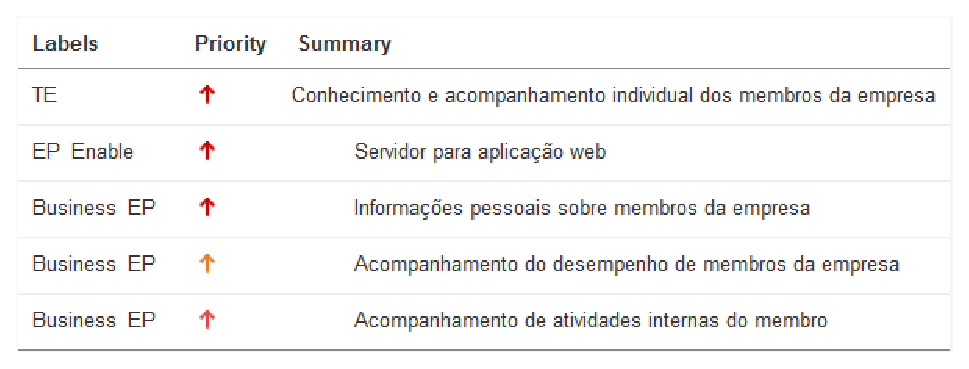
\includegraphics[keepaspectratio=true,scale=0.6]{figuras/blep01.eps}
    \caption[Backlog épicos]{Backlog priorizado de épicos\label{blep01}}
\end{figure}

\textbf{Features}

\begin{figure}[H]
    \centering
    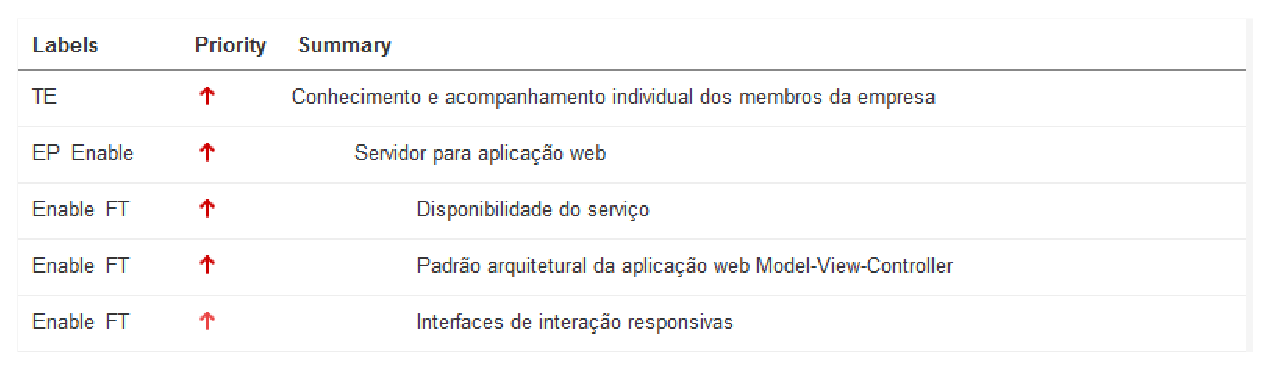
\includegraphics[keepaspectratio=true,scale=0.6]{figuras/blft01.eps}
    \caption[Backlog features]{Backlog priorizado de features\label{blft01}}
\end{figure}

\begin{figure}[H]
    \centering
    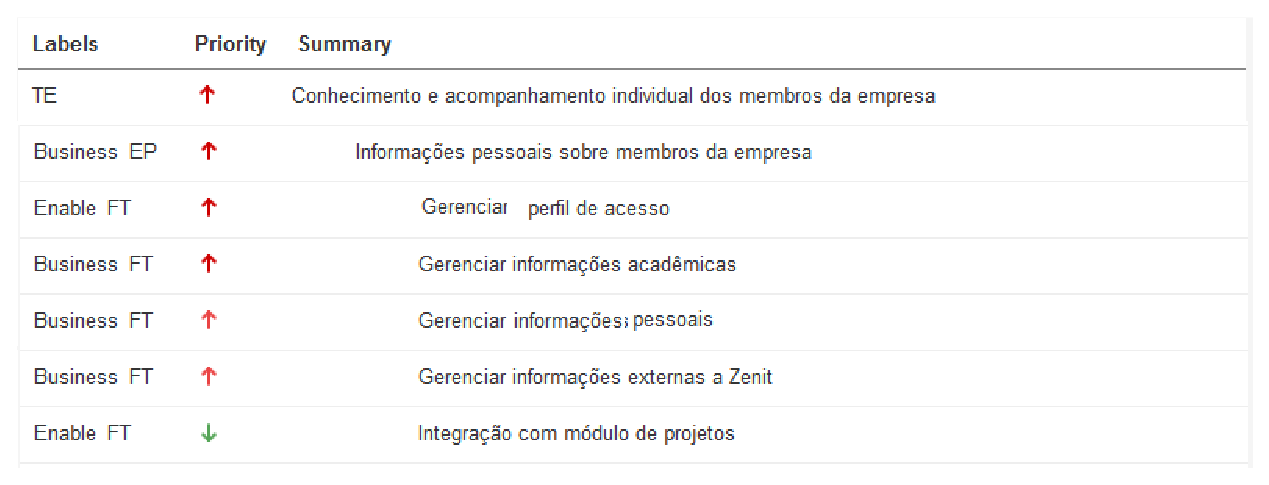
\includegraphics[keepaspectratio=true,scale=0.6]{figuras/blft02.eps}
    \caption[Backlog features]{Backlog priorizado de features\label{blft02}}
\end{figure}

\begin{figure}[H]
    \centering
    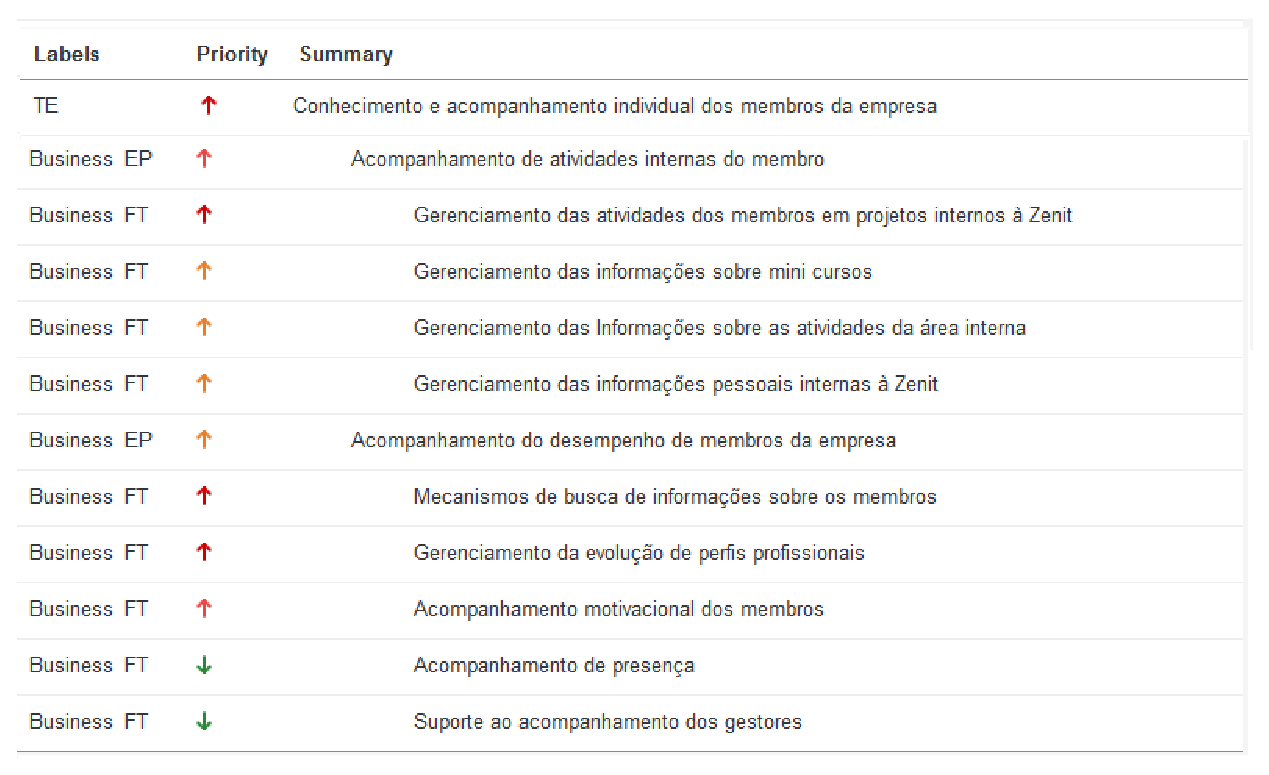
\includegraphics[keepaspectratio=true,scale=0.6]{figuras/blft03.eps}
    \caption[Backlog features]{Backlog priorizado de features\label{blft03}}
\end{figure}

\subsection{Reunião 03-Time}

 \indent \textbf{Data de execução:} 08/06/2016\\
 \indent \textbf{Objetivo da reunião:} verificar se o PO aceita as mudanças identificadas na \ref{reuniao02Time}. Elicitar histórias das features definidas no Business EP04 após mudança. \\
 \indent \textbf{Técnica de elicitação:} foi utilizada a técnica de brainstorming para identificar todas as possíveis histórias e prototipação.\\
 \indent \textbf{Execução da técnica:} com o tema de cada feature, foram jogadas ideias para histórias de usuário que atendessem a aquelas features.\\
 \indent \textbf{Resultado da reunião:} o PO concordou com todas as mudanças feitas no backlog de features e épicos.\\
 \indent Todas as histórias foram elicitadas das features “Gerenciamento das informações dos minicursos”, ”Gerenciamento das informações sobre da área interna dos membros” e ”Gerenciamento das informações internas pessoais à Zenit”, assim o objetivo da reunião foi atingido. Os protótipos gerados foram as imagens: \ref{usprototipo05}, \ref{usprototipo06}, \ref{usprototipo07}, \ref{usprototipo08}, \ref{usprototipo09}, \ref{usprototipo10}.\\
 \indent Nesta mesma reunião, o PO fez a verificação e validação das histórias. Apesar de não estar no planejamento para esta reunião, como o PO compreendeu as atividades que estavam sendo realizadas, ele sugeriu validar as histórias, assim foi feita a verificação e validação pelo PO na mesma reunião.

\begin{figure}[H]
    \centering
    \includegraphics[keepaspectratio=true,scale=0.4]{figuras/usprototipo05.eps}
    \caption[Protótipo 5 de história]{Protótipo 5 para elicitação de história\label{usprototipo05}}
\end{figure}

\begin{figure}[H]
    \centering
    \includegraphics[keepaspectratio=true,scale=0.4]{figuras/usprototipo06.eps}
    \caption[Protótipo 6 de história]{Protótipo 6 para elicitação de história\label{usprototipo06}}
\end{figure}

\begin{figure}[H]
    \centering
    \includegraphics[keepaspectratio=true,scale=0.4]{figuras/usprototipo07.eps}
    \caption[Protótipo 7 de história]{Protótipo 7 para elicitação de história\label{usprototipo07}}
\end{figure}

\begin{figure}[H]
    \centering
    \includegraphics[keepaspectratio=true,scale=0.4]{figuras/usprototipo08.eps}
    \caption[Protótipo 8 de história]{Protótipo 8 para elicitação de história\label{usprototipo08}}
\end{figure}

\begin{figure}[H]
    \centering
    \includegraphics[keepaspectratio=true,scale=0.4]{figuras/usprototipo09.eps}
    \caption[Protótipo 9 de história]{Protótipo 9 para elicitação de história\label{usprototipo09}}
\end{figure}

\begin{figure}[H]
    \centering
    \includegraphics[keepaspectratio=true,scale=0.4]{figuras/usprototipo10.eps}
    \caption[Protótipo 10 de história]{Protótipo 10 para elicitação de história\label{usprototipo10}}
\end{figure}

\subsection{Backlog de Time}

    Este backlog a nível de time já está de acordo com as mudanças descritas na seção anterior, estão priorizadas de acordo com os interesses do \textit{Product Owner} e após a análise da equipe. No \autoref{especUs} contém todas as especificações das histórias.

\begin{figure}[H]
    \centering
    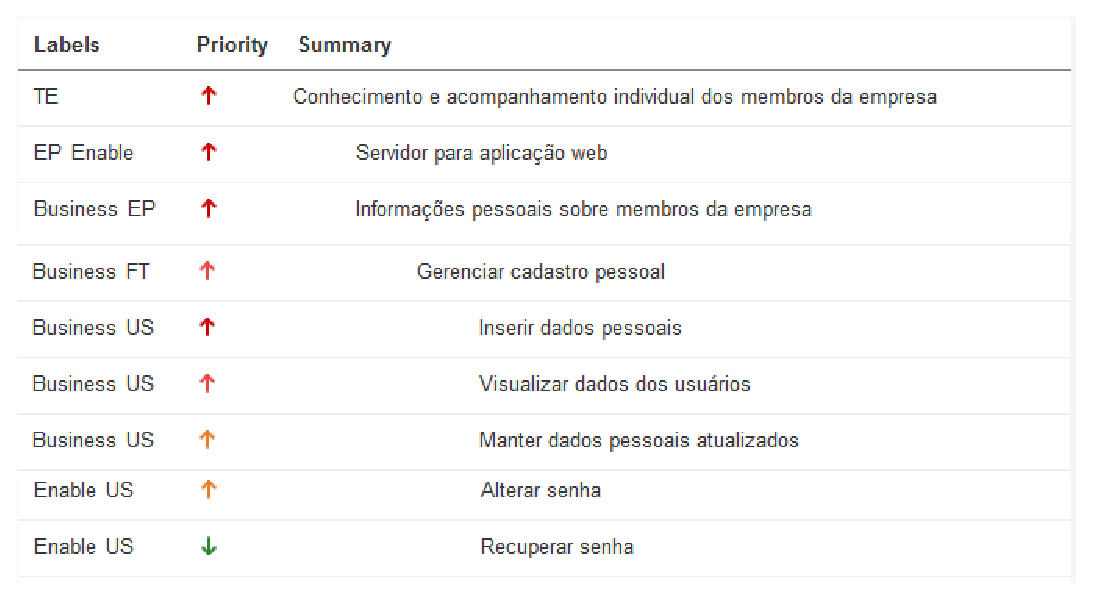
\includegraphics[keepaspectratio=true,scale=0.6]{figuras/blus01.eps}
    \caption[Backlog história]{Backlog priorizado de histórias\label{backlogus01}}
\end{figure}

\begin{figure}[H]
    \centering
    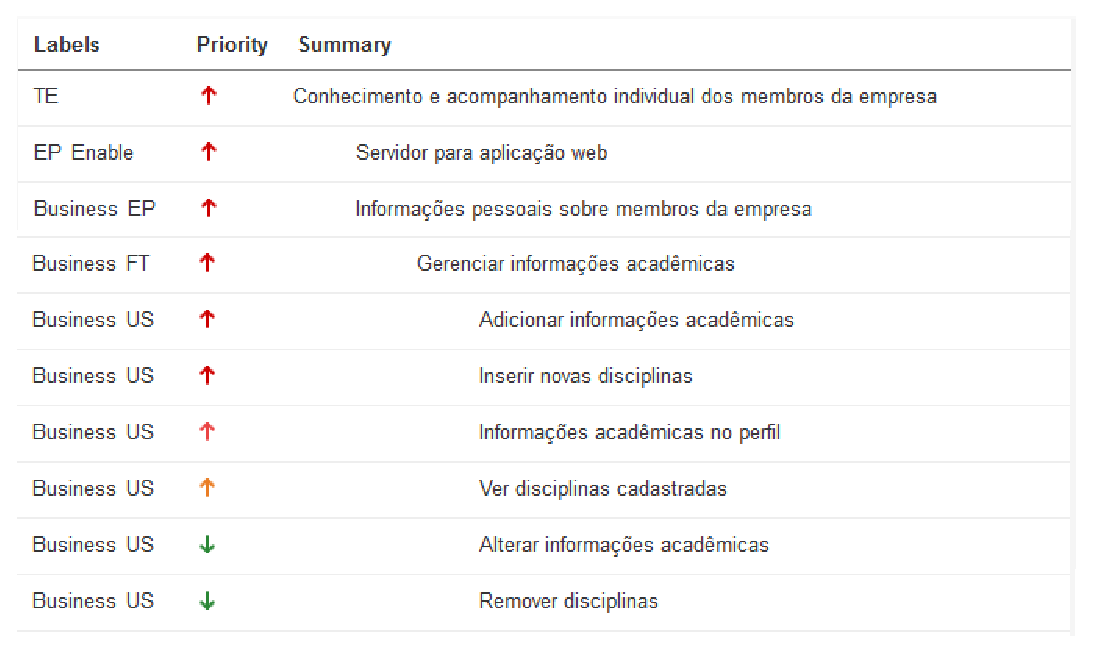
\includegraphics[keepaspectratio=true,scale=0.6]{figuras/blus02.eps}
    \caption[Backlog história]{Backlog priorizado de histórias\label{backlogus02}}
\end{figure}

\begin{figure}[H]
    \centering
    \includegraphics[keepaspectratio=true,scale=0.6]{figuras/blus03.eps}
    \caption[Backlog história]{Backlog priorizado de histórias\label{backlogus03}}
\end{figure}

\begin{figure}[H]
    \centering
    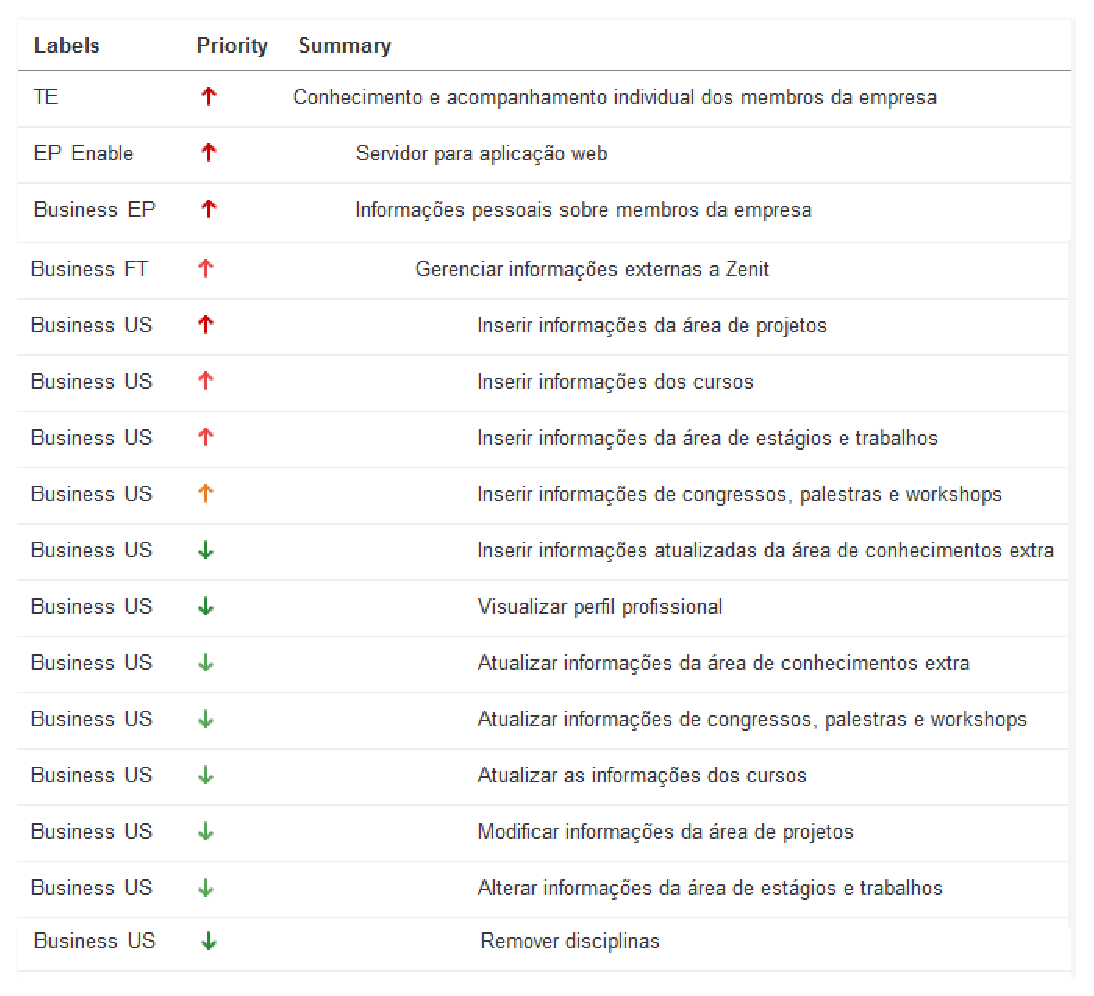
\includegraphics[keepaspectratio=true,scale=0.6]{figuras/blus04.eps}
    \caption[Backlog história]{Backlog priorizado de histórias\label{backlogus04}}
\end{figure}

\begin{figure}[H]
    \centering
    \includegraphics[keepaspectratio=true,scale=0.6]{figuras/blus05.eps}
    \caption[Backlog história]{Backlog priorizado de histórias\label{backlogus05}}
\end{figure}

\begin{figure}[H]
    \centering
    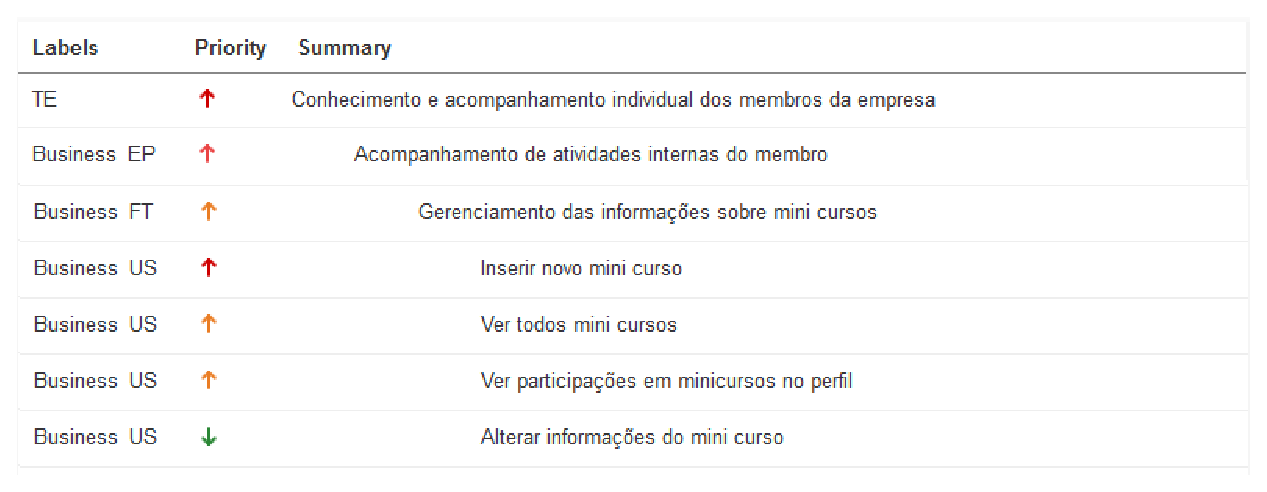
\includegraphics[keepaspectratio=true,scale=0.6]{figuras/blus06.eps}
    \caption[Backlog história]{Backlog priorizado de histórias\label{backlogus06}}
\end{figure}

\begin{figure}[H]
    \centering
    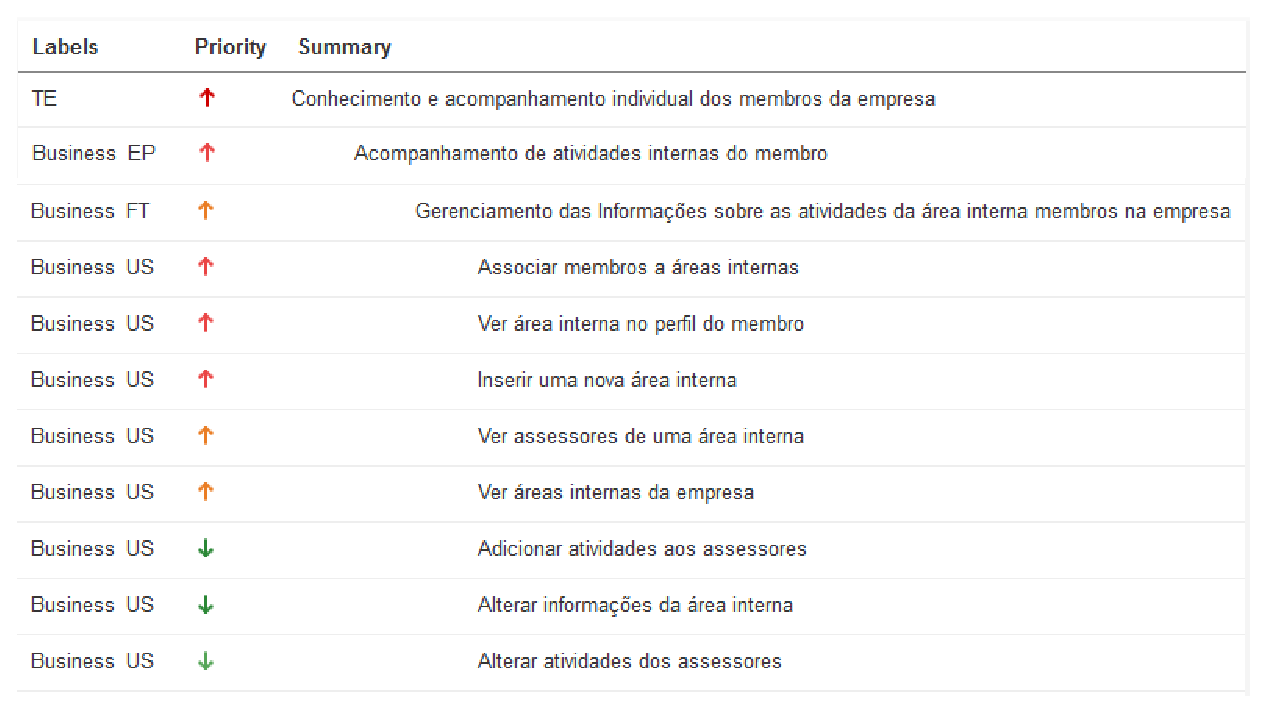
\includegraphics[keepaspectratio=true,scale=0.6]{figuras/blus07.eps}
    \caption[Backlog história]{Backlog priorizado de histórias\label{backlogus07}}
\end{figure}

\begin{figure}[H]
    \centering
    \includegraphics[keepaspectratio=true,scale=0.6]{figuras/blus08.eps}
    \caption[Backlog história]{Backlog priorizado de histórias\label{backlogus08}}
\end{figure}

\section{Planejamento da sprint}

\begin{figure}[H]
    \centering
    \label{identificarPlanejar}
    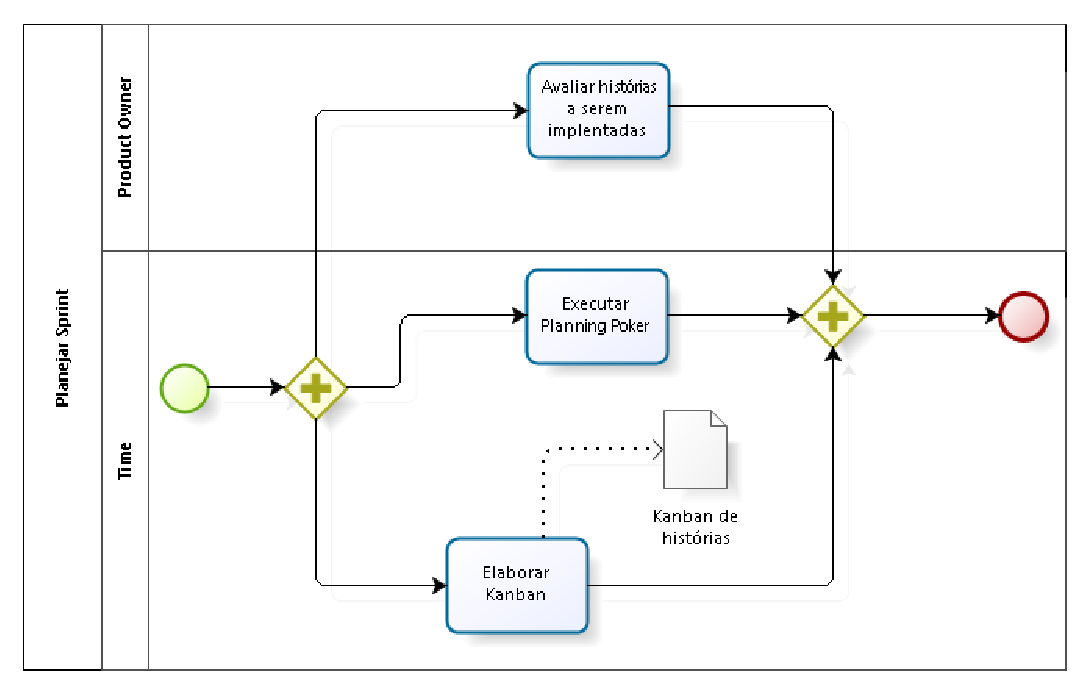
\includegraphics[keepaspectratio=true,scale=0.6]{figuras/processoPlanejar.eps}
    \caption[Planejar sprint]{Processo - Nível de Time - Planejar sprint}
\end{figure}

\subsection{Reunião 04-Time}

Foi feita uma reunião interna, somente com os membros da equipe de requisitos, para realizar o planejamento da sprint 01, foi analisado com base na prioridade determinada pelo PO de qual épico e feature as histórias de usuários seriam selecionadas para serem implementadas. Foi levado em consideração também a produtividade e perfil da equipe. Com base nesses critérios, foram determinados as histórias de usuário a serem implementadas. 

Sendo estas as histórias de usuário, da imagem \ref{blft01} selecionadas para serem implementadas: 


\begin{figure}[H]
    \centering
    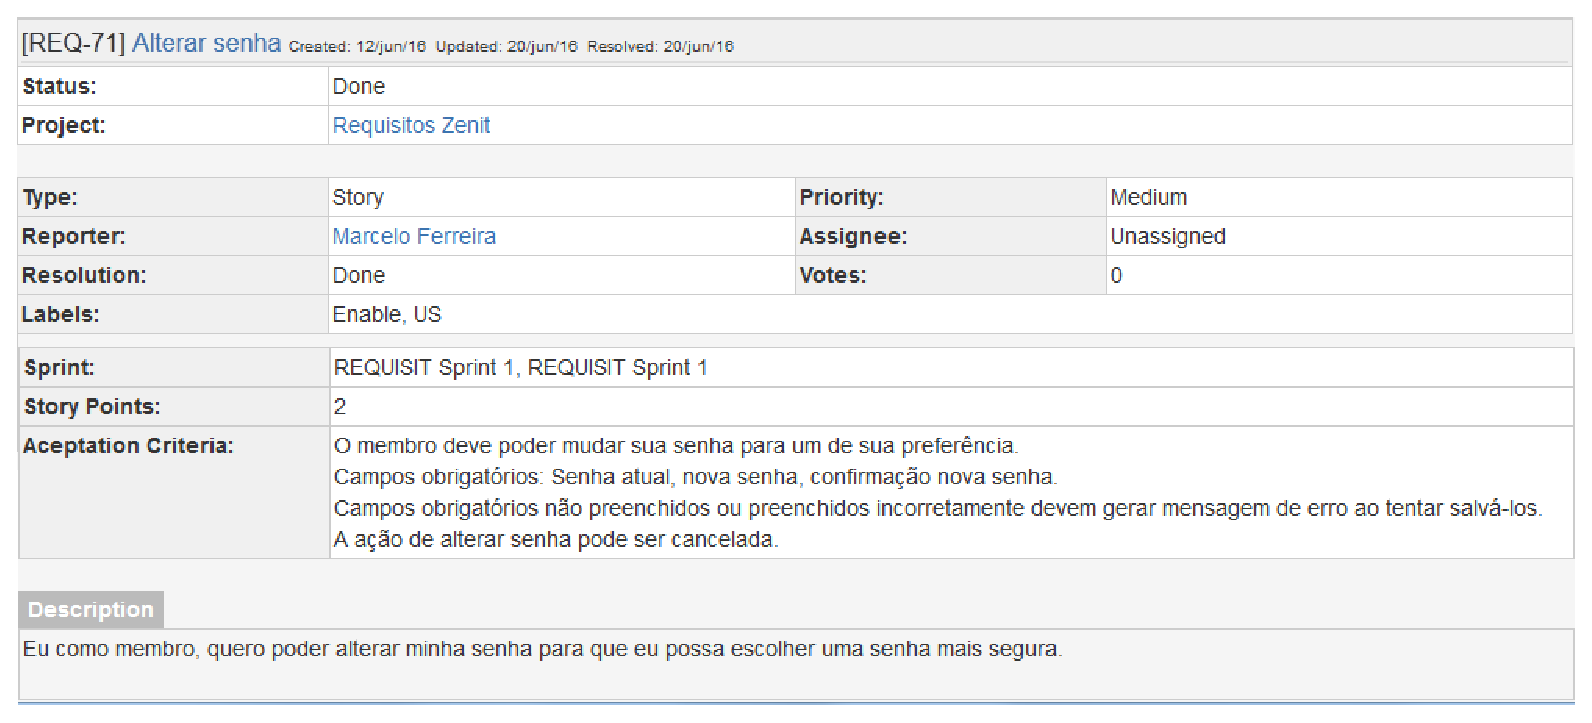
\includegraphics[keepaspectratio=true,scale=0.6]{figuras/us01.eps}
    \caption[História da sprint 01]{História para execução da sprint01}
\end{figure}

\begin{figure}[H]
    \centering
    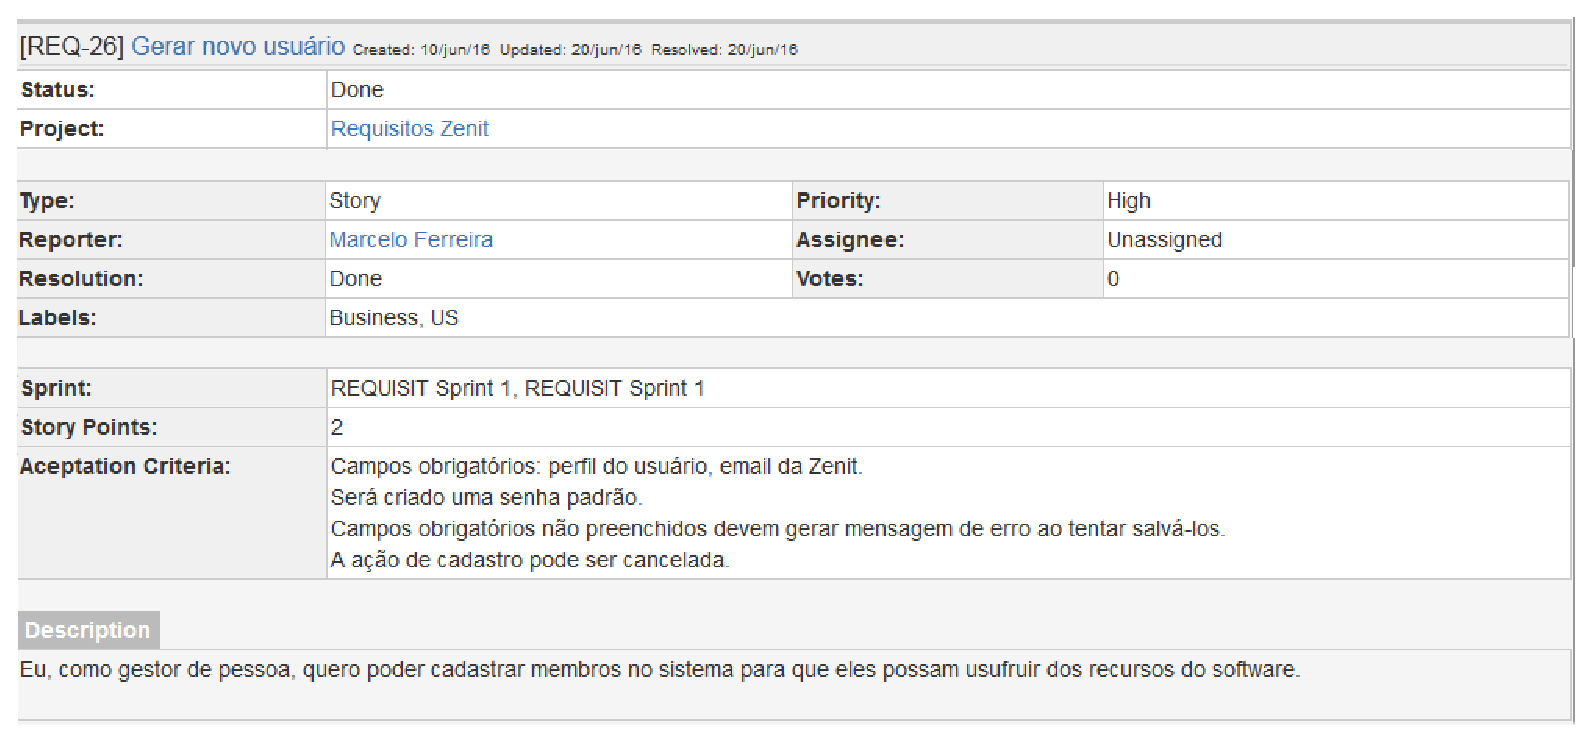
\includegraphics[keepaspectratio=true,scale=0.6]{figuras/us02.eps}
    \caption[História da sprint 01]{História para execução da sprint01}
\end{figure}

\begin{figure}[H]
    \centering
    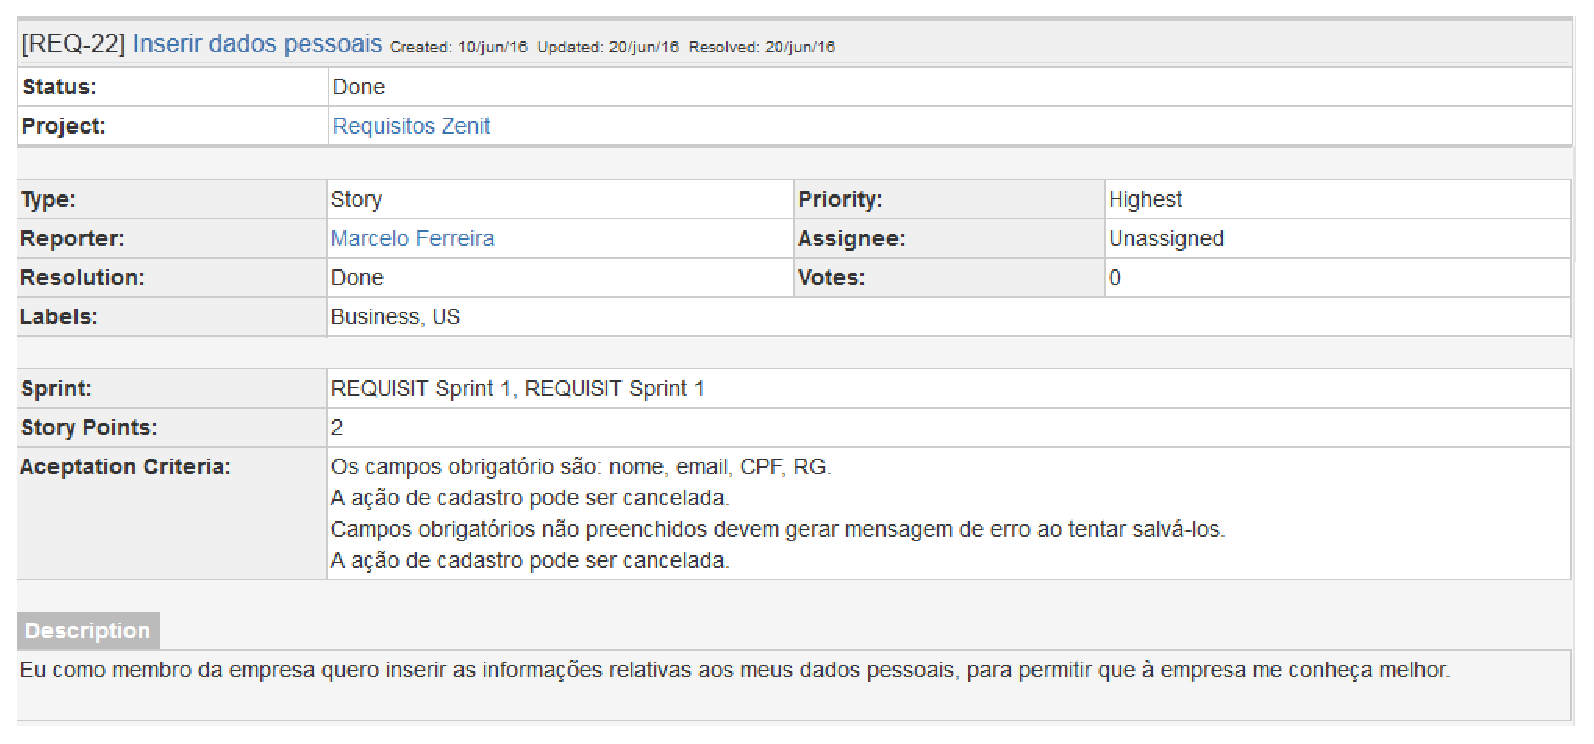
\includegraphics[keepaspectratio=true,scale=0.6]{figuras/us03.eps}
    \caption[História da sprint 01]{História para execução da sprint01}
\end{figure}
\begin{figure}[H]
    \centering
    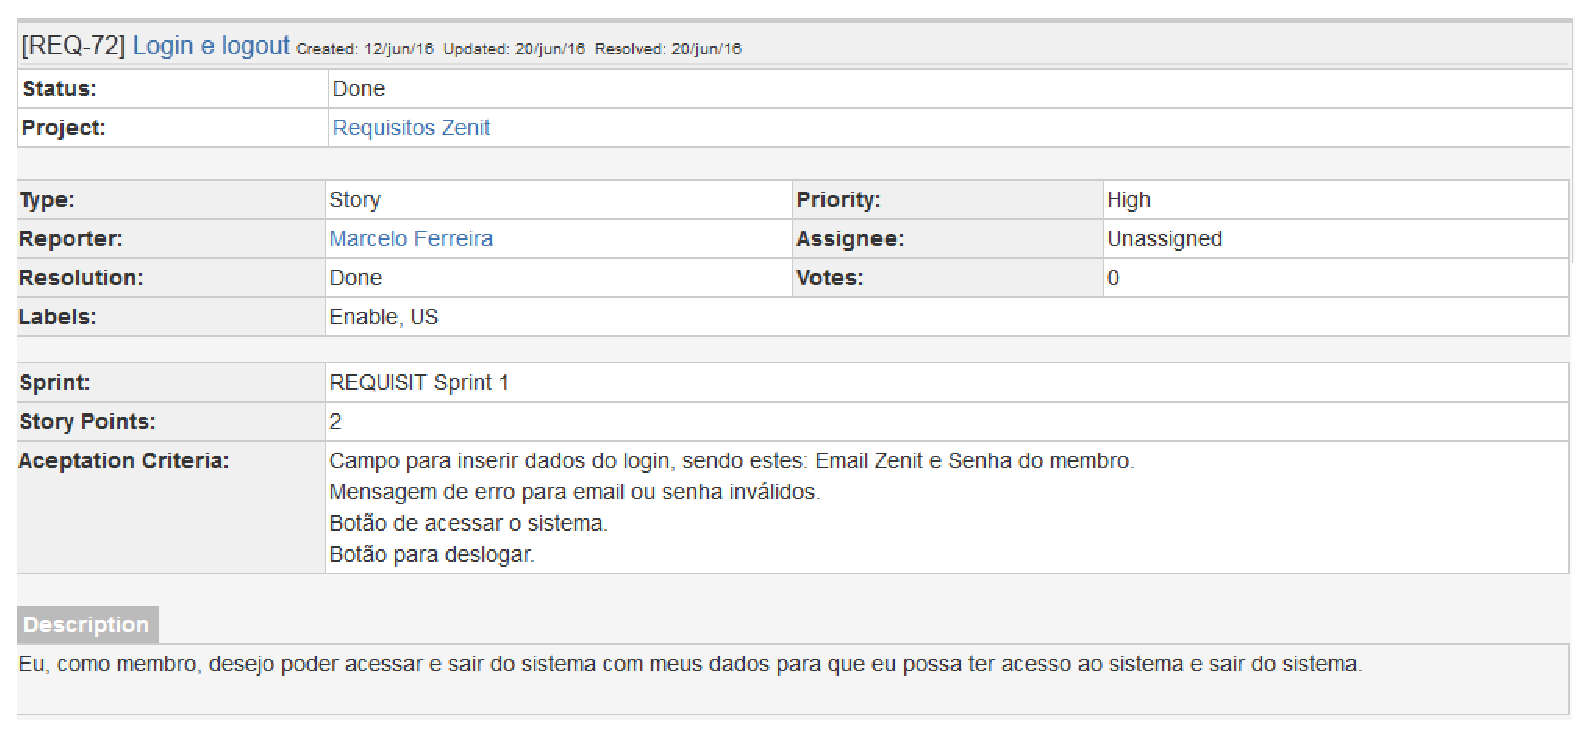
\includegraphics[keepaspectratio=true,scale=0.6]{figuras/us04.eps}
    \caption[História da sprint 01]{História para execução da sprint01}
\end{figure}
\begin{figure}[H]
    \centering
    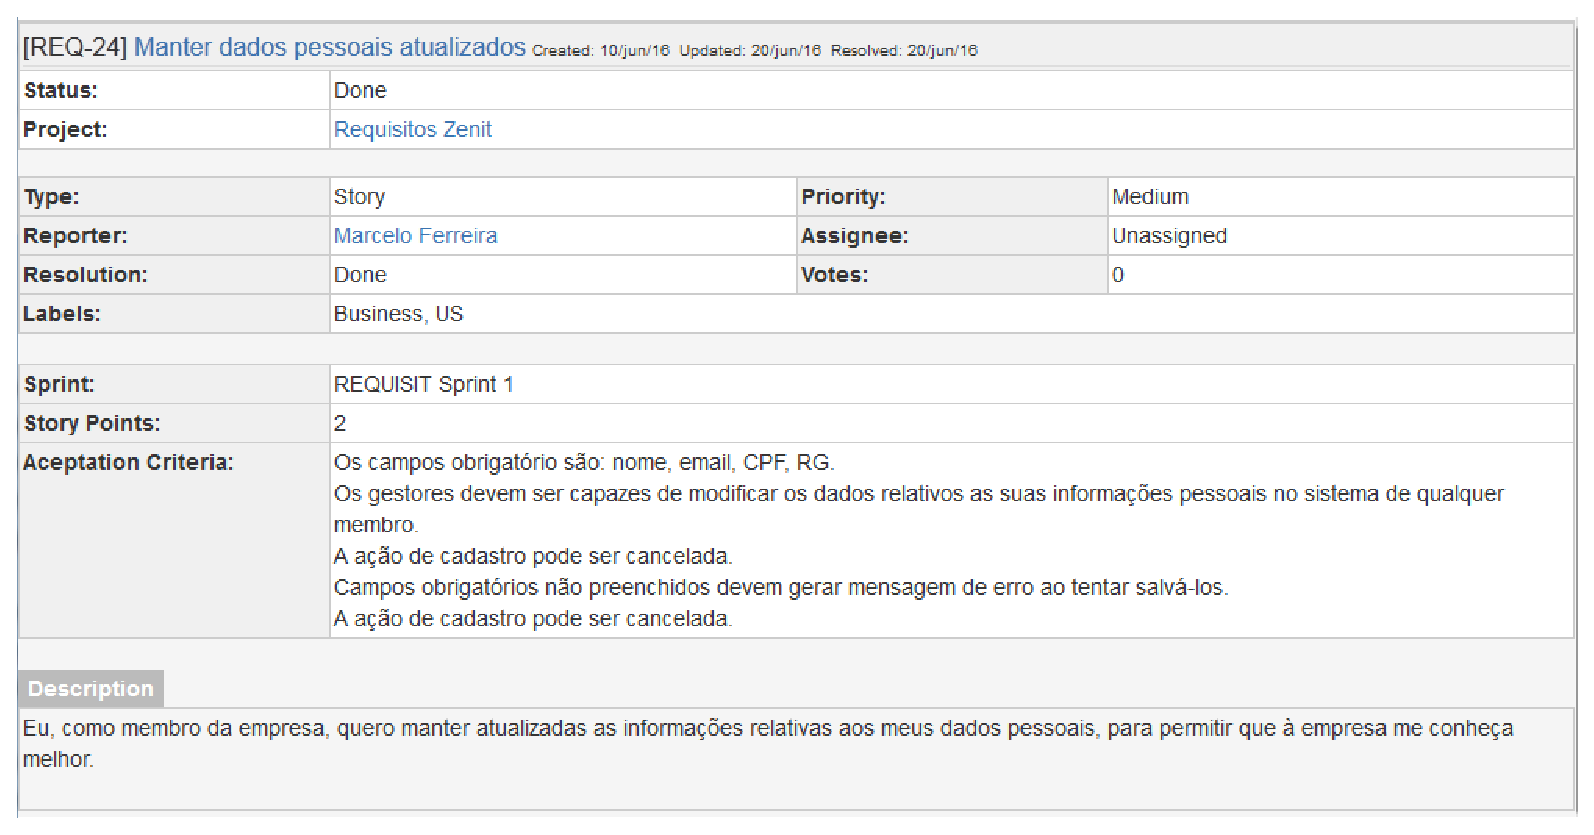
\includegraphics[keepaspectratio=true,scale=0.6]{figuras/us05.eps}
    \caption[História da sprint 01]{História para execução da sprint01}
\end{figure}
\begin{figure}[H]
    \centering
    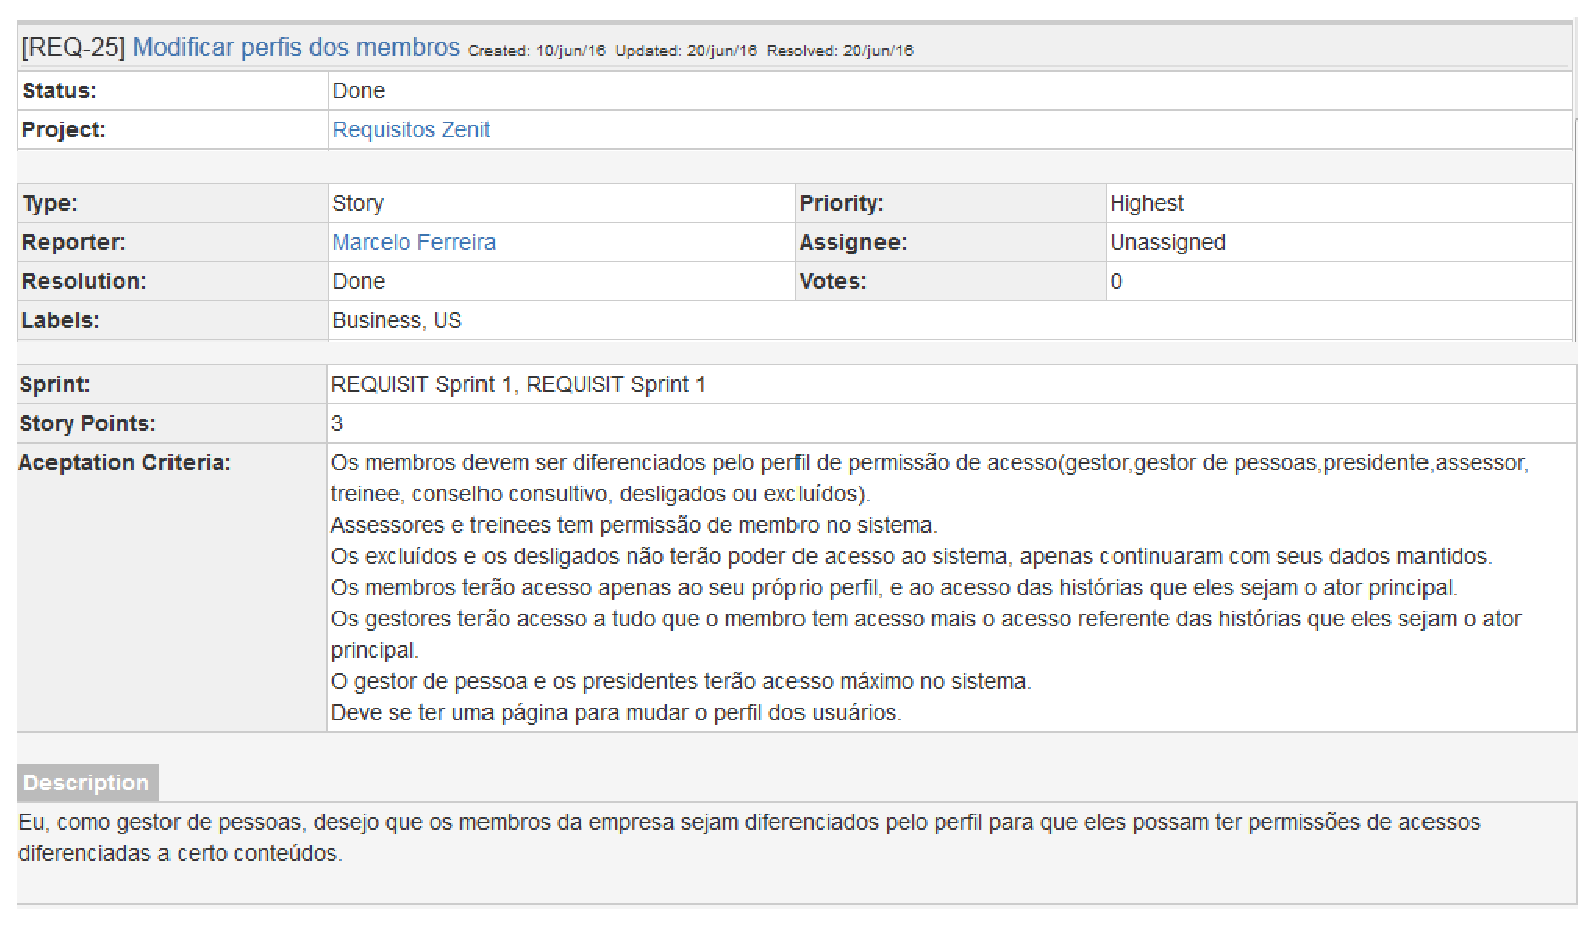
\includegraphics[keepaspectratio=true,scale=0.6]{figuras/us06.eps}
    \caption[História da sprint 01]{História para execução da sprint01}
\end{figure}
\begin{figure}[H]
    \centering
    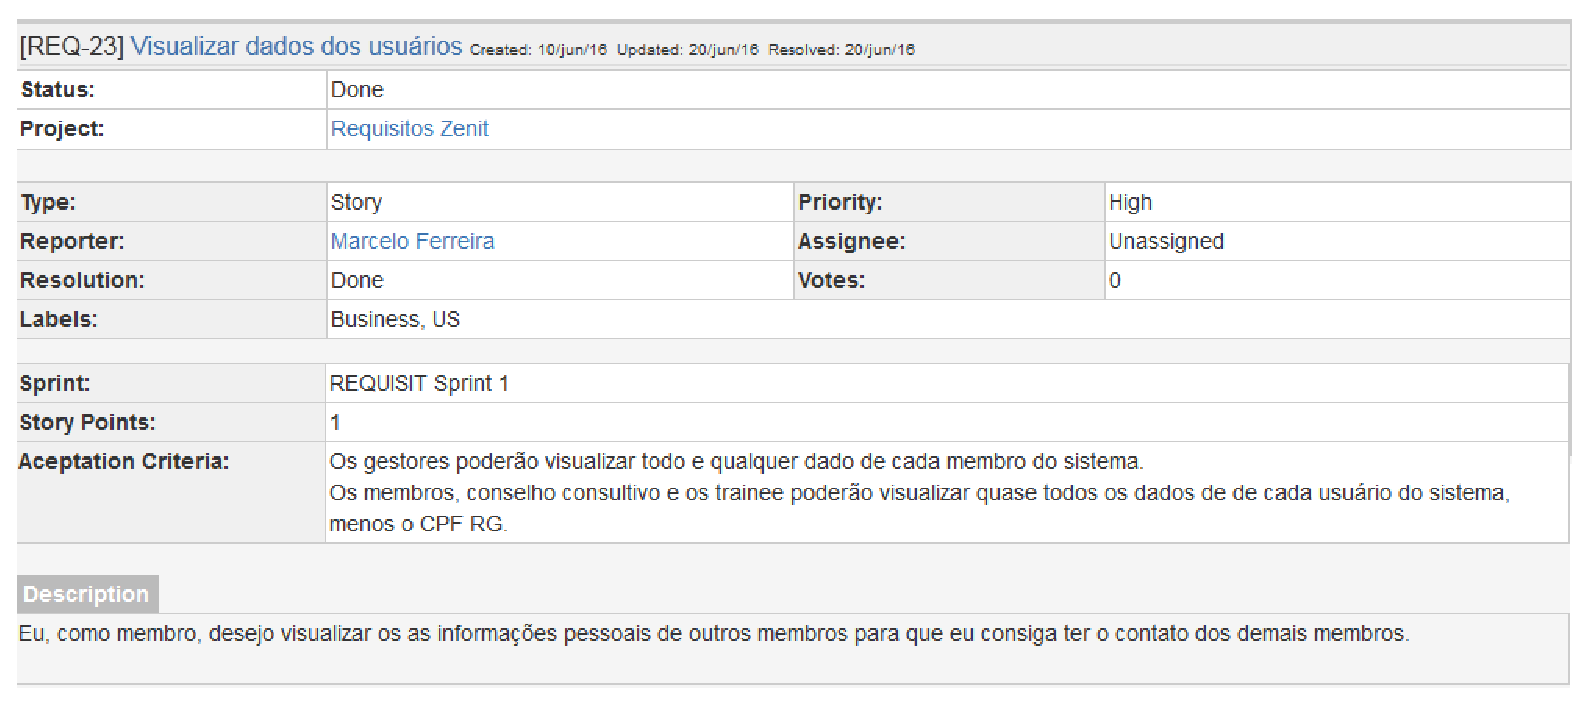
\includegraphics[keepaspectratio=true,scale=0.6]{figuras/us07.eps}
    \caption[História da sprint 01]{História para execução da sprint01\label{usPontoUm}}
\end{figure}

Com as histórias de usuário selecionadas, foi realizado o plannig poker e foi determinado que a história de Visualizar dados dos usuários \ref{usPontoUm} seria nosso parâmetro para definir complexidade da história, sendo esta equivalente ao ponto 01, baseando-se nas experiências dos membros da equipe de requisitos. Logo, as pontuação das histórias foram: 

\begin{table}[H]
    \centering
    \label{historiasImplementar}
    \caption{Histórias pontuadas para implementação}
    \begin{tabular}{|l|l|}
        \hline
        US & Pontuação\\
        \hline
        Manter dados pessoais atualizados & 02\\
        \hline
        Inserir dados pessoais &  02\\
        \hline
        Visualizar dados dos usuários & 01\\
        \hline
        Modificar perfis dos membros & 03\\
        \hline
        Gerar novo usuário & 02\\
        \hline 
        Login / logout & 02\\
        \hline
    \end{tabular}
\end{table}

\section{Execução da sprint}

\begin{figure}[H]
    \centering
    \label{identificarExecutar}
    \includegraphics[keepaspectratio=true,scale=0.6]{figuras/processoExecutar.eps}
    \caption[Executar sprint]{Processo - Nível de Time - Executar sprint}
\end{figure}

\textbf{Execução da sprint:} 11/06/2016 à 18/06/2016

No desenvolvimento das histórias de usuários houveram dificuldades da equipe de requisitos em desenvolver as histórias de usuário, uma vez que, um dos membros da equipe não havia conhecimento sobre a linguagem e ferramentas escolhidas para o desenvolvimento, Ruby on Rails e suas demais Gems, e um dos membros ficou sem computador deixando assim a equipe de desenvolvimento desfalcada durante a execução da sprint 01.

O backlog da sprint 01 foi concluída, ou seja, todas as funcionalidade foram entregues. Porém, por conta de dificuldades na utilização da ferramenta com relação aos frameworks de layout, houve uma divida técnica em relação ao layout das histórias de usuários. Logo, a usabilidade do layout das USs não esta inadequada.

\subsection{Resumo da sprint}

Ao final do término da sprint 01, foi realizada uma reunião, dia 19/06/2016, para realizar a retrospectiva e revisão da sprint. Ao final da reunião, foi gerado um documento, que está no \autoref{resumoSprint},contendo os pontos bons e ruins e melhorias para as próximas sprints.

\begin{table}[H]
    \centering
    \caption{Tabela resumo}
    \label{tabelaResumoSprint}
    \begin{tabular}{|c|p{10cm}|}
        \hline
        \textbf{Bom} & \textbf{Ruim} \\
        \hline
        Apredizado das ferramentas  &  Membros não trabalharam \\
        & Membro sem notebook durante a sprint \\
        & Membro com desconhecimento da linguagem e ferramentas utilizadas\\
        &  Entregas de outras disciplinas e não houve pareamento \\
        &  Atraso de entrega\\
        &  Dificuldade com a ferramenta\\
        & Dificuldade com a linguagem\\
        \hline
        \multicolumn{2}{|c|}{\textbf{Melhorias}}\\
        \hline
        \multicolumn{2}{|c|}{Maior interação entre os membros} \\
        \multicolumn{2}{|c|}{Fazer pareamento} \\
        \multicolumn{2}{|c|}{Dividir melhor as histórias} \\
        \multicolumn{2}{|c|}{Melhorar planejamento da sprint} \\
        \hline
    \end{tabular}
\end{table}

